\chapter{Tesztelés}
Ebben a fejezetben az elkészített megoldó algoritmus tesztelését mutatom be, hogy az megfelelően, hiba nélkül képes a feladatokat megoldani.
A tesztelés a következő konfigurációval rendelkező számítógéppel történt:
\begin{itemize}
	\item Processzor: Intel i5-7200, 2,50 Ghz
	\item 8 GB RAM
	\item Operációs rendszer: Windows 10
	\item Fejlesztési használt szoftverek:
		\begin{itemize}
			\item Qt Creator 4.7.1
			\item Qt 5.11.2
			\item Boost Libraries 1.68.0
			\item Microsoft Visual C++ Compiler 15.0 
		\end{itemize}		 
\end{itemize}

Az S-gráf megoldó szoftvert parancssori paraméterek segítségével lehet működtetni. A különböző megoldó módszereket, amelyek megtalálhatóak a szoftverbe implementálva, más és más kapcsolók segítéségével lehet elérni, meghívni. Ezeknek listája megtalálható a \textbf{solver} mappában lévő \textbf{README.md} fájlban. Az általam megvalósított módszerhez a következő kapcsolókat mindenképpen használni kell, hogy a program hiba nélkül fusson, végezze el az ütemezést.
\begin{itemize}
	\item \textbf{-i extended\textunderscore precedential.ods:} A bemeneti fájl elérési útvonalát kell megadni ezzel.
	\item \textbf{-o output.txt:} A kimeneti fájl elérési útvonala. Két fajta kiterjesztésű fájlt lehet megadni: \textbf{TXT} és \textbf{PNG}. Előbbi esetében a fájlba kerülnek az élek, mind a recepet, mind az ütemezési élek, valamint, hogy mennyi ideig tart a részfeladat befejezése, amelyből ezek kiindulnak. Ezenfelül a Gantt diagram karakteres formában is megjelenik. PNG kiterjesztésű fájl megadása esetén pedig kirajzolásra kerül egy Gantt diagram
	\item \textbf{-m flexbatch:} Ezzel a kapcsolóval a megoldó módszert lehet kiválasztani. A \textit{felxbatch} határozza meg, hogy az általam megvalósított algoritmus kerüljön meghívásra.
	\item \textbf{--timehor:} Időhorizont megadása történik ezzel a kapcsolóval
	\item \textbf{--obj profit\textunderscore max:} A célfüggvény kiválasztása, ebben az esetben az újonnan a megoldószoftverhez hozzáadott profit maximalizálás kerül kiválasztásra.
	\item \textbf{--precycle off:} Az precycle az ütemezés gyorsításra szolgál, mégpedig úgy, hogy előre lefut, és kört keres a gráfban. Az új módszer esetén hibásan működik, nem összeegyeztethető azzal, ezért szükséges a kikapcsolása.
	\item \textbf{--nopresolvers:} Hasonlóan az előzőhöz a presolver is az ütemezést gyorsítja, de nem egyeztethető össze az új megoldó módszerrel, emiatt kell mindenképpen inaktívvá tenni.
\end{itemize}

A ~\ref{teszFeladat} ábrán látható mintafeladat alapján kerül bemutatásra a megoldó módszer. Két termékhez tartozó receptet látunk, illetve a részfeladatokat, valamint az ezeket megvalósítani képes berendezéseket. Az éleken megfigyelhetőek még a taszkok befejezéséhez szükséges idő.
\begin{figure}[H]
\begin{center}
\includegraphics[scale=0.7]{tesztfeladat}
\caption{Tesztfeladat}
\label{teszFeladat}
\end{center}
\end{figure}

\section{Taszkok közötti kapacitások változtatásának hatása}
A módszer sajátossága, hogy a receptélekkel az egyes taszkok kapacitásának meghatározott százaléka hasznosítható. Ezeket a százalékokat a bemeneti fájlban lehet megadni. A példafeladat a~\ref{bemenet1} ábrán megtekinthető bemeneti adatokkal rendelkezik. Az időhorizont a bemutatott mintafeladat során 20. Látható, hogy az egyes részfeladat által lehetséges kapacitásoknak nem a teljes mennyisége kerül tovább a következő köztes feladathoz. Ez, hogy kisebb mennyiség kerül felhasználásra nagy mértékben befolyásolja a korlátot. Emellett az ütemezés megoldását is befolyásolja, mert emiatt lehetséges, hogy bizonyos berendezések nem végezhetik el az adott taszkot.

Az egyszerűség kedvéért a példában csak 2 darab A terméket és 1 darab B terméket gyártunk le. Mindkét termék legyártásából származó jövedelem mindössze egy egység. A \textit{precendce} táblában látható, hogy a taszkok által elérhető mennyiségek nem 100 százalékban kerülnek további felhasználása. Például az A1 és A2 taszkok esetében, az A1-es taszk mennyiségének 80 százaléka kerül továbbítása, illetve ennek a már kisebb mennyiségnek a 70 százalékát veszi fel az A2-es részfeladat. A \textit{proctime} táblán megtalálhatjuk, hogy melyik taszkot, melyik berendezés tudja elvégezni, valamint ezt mennyi idő alatt.
 
\begin{figure}[H]
\begin{center}
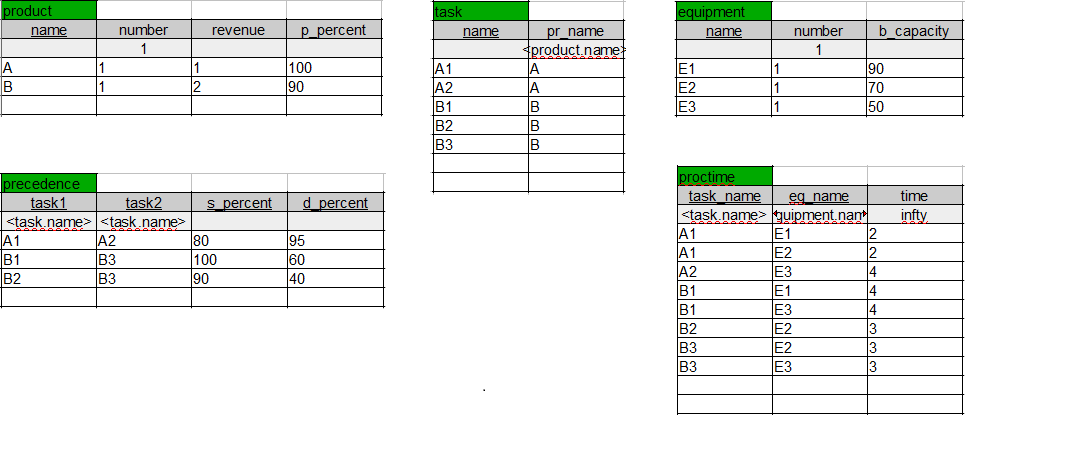
\includegraphics[scale=0.7]{bemenet1}
\caption{Első feladat bemeneti adatai}
\label{bemenet1}
\end{center}
\end{figure}

A feladat megoldását tartalmazó TXT kiterjesztésű fájlt három darab elkülöníthető részre tudjuk felosztani. Az első része látható a~\ref{eredmeny1} ábrán. Az ábra elején az éleket találhatjuk meg, mégpedig olyan formában, hogy melyik taszkból melyik taszkba mutat. Továbbá láthatók idő értékek, amelyek megadják, hogy az élt megelőző részfeladatot mennyi idő alatt lehet elvégezni. Ez a rész tartalmazza mind a receptéleket, mind az ütemezési éleket. Úgy tudjuk ezeket elkülöníteni, hogy amelyikhez 0 időérték van rendelve, azok tartoznak a az ütemezési élek csoportjához. Mivel az egyik termékből, nevezetesen az A-ból, több mint egy darabot gyártunk ezért megkülönböztetjük az egyes receptekhez tartozó feladatokat. Láthatunk A1-et és A1\textunderscore 2-t. Ugyanolyan típusú feladatról beszélünk, de különböző recepthez tartoznak, ezért kell megkülönböztetni egymástól ezeket. 
\begin{figure}[H]
\begin{center}
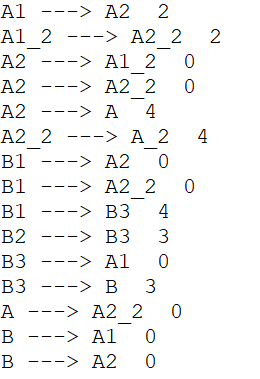
\includegraphics[scale=0.8]{eredmeny1}
\caption{A megoldást tartalmazó fájl első része}
\label{eredmeny1}
\end{center}
\end{figure}
A második részben a taszkok és a hozzájuk tartozó kapacitások, valamint a termékekhez tartozó kapacitások és a termékek előállításából származó jövedelem szorzata található. Ezeket követően szerepel a bound, a korlát, ami az adott feltételek és adatok mellett 173,846 lett. Ezt úgy kapjuk meg, hogy a termékekhez tartozó értékeket összeadjuk. Jelen példa esetében 3 érték kerül összeadásra, ezek a következők: A2, A2\textunderscore 2, és a B3. Az A2-es és a A2\textunderscore 2-es részfeladatok kapacitása 60, a B3-as taszk kapacitása pedig 53,846. Mivel a példában mindkét termék esetében a jövedelem egy, ezért az érték marad változatlanul a termékeknél. Ezeket összeadva kijön a 173,846, ami megegyezik a szoftver által kiszámolt megoldással. Ezek az értékek a~\ref{eredmeny2} ábrán megtekinthetőek.
\begin{figure}[H]
\begin{center}
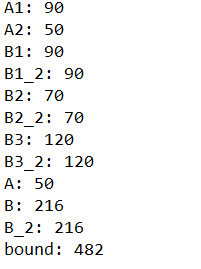
\includegraphics[scale=0.85]{eredmeny2}
\caption{A megoldást tartalmazó fájl második része}
\label{eredmeny2}
\end{center}
\end{figure}
Az utolsó szakaszban a Gantt diagram karakteres formában található meg. Látható, hogy a megadott bemeneti adatok alapján minden lehetséges taszk és berendezés kombináció elő áll. A\ref{eredmeny3} ábrán látható ez. 
\begin{figure}[H]
\begin{center}
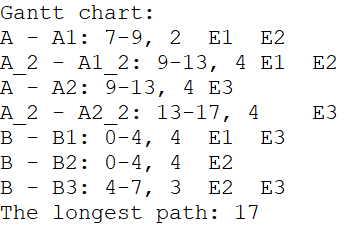
\includegraphics[scale=0.85]{eredmeny3}
\caption{A megoldást tartalmazó fájl második része}
\label{eredmeny3}
\end{center}
\end{figure}
A következő esetben újra lefuttatjuk a példafeladatot, azzal a kis változtatással a bemeneti adatokon, hogy az élekhez tartozó százalékok mindegyikét felemeljük 100 százalékra, vagyis a teljes mennyiség minden taszk esetében tovább kerül a következő részfeladathoz. A többi adat, köztük a kapcsolóval megadott idő horizont is változatlan marad. 

Ahogy várható volt az újbóli futtatás során eltérések vannak az előzőhöz képest. Egyik legfontosabb eltérése, hogy a bound megváltozott. Ebben az esetben már csak 170 lett. A jelenlegi futás során a bound kereken 170 lesz. További eltérése, hogy most már nem minden lehetséges taszk - berendezés pár lett összerendelve, mert abban az esetben a megadott idő horizonton belül nem lenne megoldható a feladat. A változás a B3-as taszk esetében történt meg. Az E3-as berendezés már nem lett hozzárendelve, azaz ezt a feladatot nem végzi el. A megoldó szoftver által elkészített png kiterjesztésű fájl látható a~\ref{output2} ábrán. Könnyen leolvasható, hogy a berendezések párhuzamosan képesek ugyanazt a taszkot elvégezni. Erre példa a B1-es köztes feladat rögtön az ütemezés elején. 

\begin{figure}[H]
\begin{center}
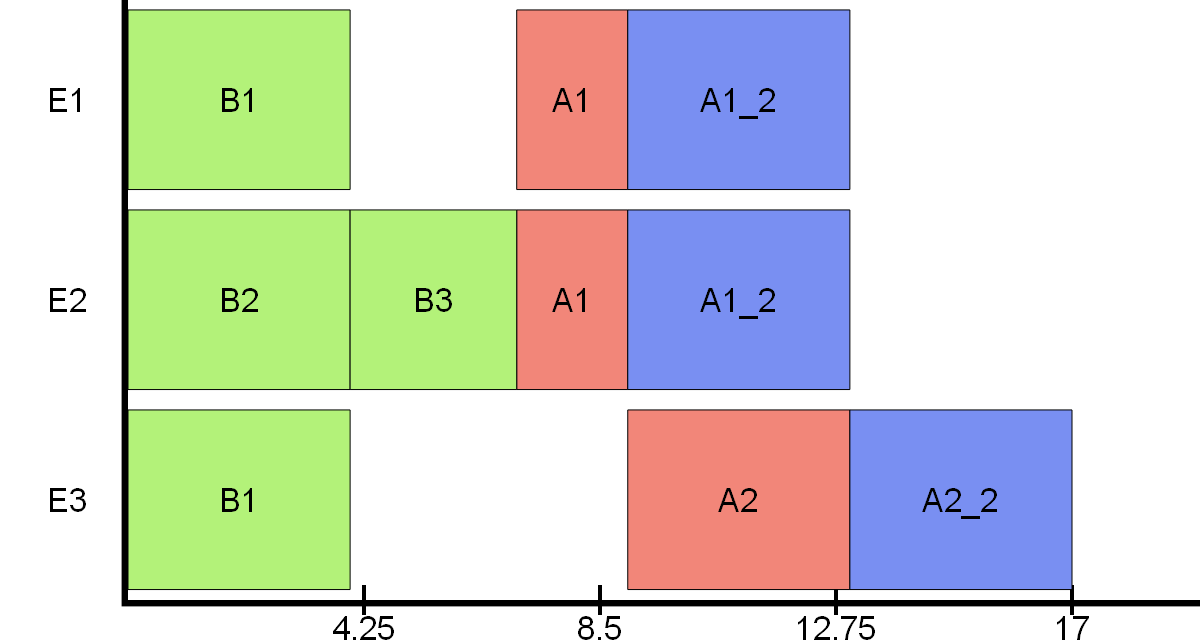
\includegraphics[scale=0.5]{output2}
\caption{A solver által elkészített Gantt diagram}
\label{output2}
\end{center}
\end{figure}

\section{Idő horizont változtatás}
A parancssori paraméterben megadott idő horizont is fontos szerepet tölt be az ütemezés során. Az eddig bemutatott példáknál nem változott meg. Ebben a részben viszont ennek a változtatására bekövetkező változások bemutatása a cél.

\begin{table}[H]
	\begin{center}
		\caption{Adott időhorizont alatt elérhető bevételek}
  		\captionsetup[table]{skip=10pt}
    	\label{tab:table2}
		\begin{tabular}{|c|c|c|c|c|c|c|c|}
		\hline
		Idő horizont & \textless =11 & 12 & 13 & 14 & 15 & 16 & \textgreater =17\\
		\hline
		Max bevétel & nem megoldható & 139,048 & 153,333 & 155.714 & 159,56 & 159,56 & 173,846\\
		\hline
		\end{tabular}	
	\end{center}
	
\end{table}

IDE TERVEZEK EGY TÁBLÁZATOT AMIBEN NÖVELEM A TERMÉKEK SZÁMÁT, ÉS A FONTOSABB ADATOKAT TÁROLNI BENN, EZÁLTAL ÖSSZEHASONLÍTHATÓVÁ VÁL